\documentclass{article}
\usepackage{graphicx}
\usepackage[utf8]{ctex}
\usepackage{amsmath}
\usepackage[fontsize=10pt]{fontsize}
\usepackage{geometry}
\geometry{a4paper,left=0.75in,right=0.75in,top=1in,bottom=0.75in}
\usepackage{setspace}
\setlength{\parindent}{0em}
\def\kong{\hspace*{2em}}
\usepackage{amsfonts,amssymb}
\usepackage{xcolor}
\usepackage{fontspec}
\usepackage{enumitem}
\linespread{1.5}
\usepackage{hyperref}
\usepackage{hyperref}
\usepackage{multirow}
\hypersetup{hidelinks,
	colorlinks=true,
	allcolors=black,
	pdfstartview=Fit,
	breaklinks=true}

\usepackage{listings}
	\lstset{
 columns=fixed,
 numbers=left,
 numberstyle=\tiny\color{gray},
 frame=none,
 backgroundcolor=\color[RGB]{245,245,244},
 keywordstyle=\color[RGB]{40,40,255},
 numberstyle=\footnotesize\color{darkgray},
 commentstyle=\it\color[RGB]{0,96,96},
 stringstyle=\rmfamily\slshape\color[RGB]{128,0,0},
 showstringspaces=false,
 language=c,
 basicstyle=\ttfamily
	}

\usepackage{fancyhdr}

\pagestyle{fancy}
\fancyhf{}
\fancyhead[LE,RO]{\thepage}
\fancyhead[RE,LO]{\kaishu PB21000276施耀炜}



\date{2022年3月}

\begin{document}

\setcounter{page}{1}
\thispagestyle{empty}
\kong
\\[10pt]
\begin{center}
	\textbf{\huge \heiti 实验报告六}\\[6pt]
    \textbf{\huge \heiti 光电效应数据处理}\\[12pt]
	\textbf{学号：}\underline{\kaishu PB21000276} \qquad 
    \textbf{姓名：}\underline{\kaishu 施耀炜} \qquad 
    \textbf{班级：}\underline{\kaishu 21级少院6班}\qquad 
    \textbf{日期：}\underline{2022年5月11日}\\[24pt]
\end{center}
\section{数据处理与分析}
    \subsection{不同光照测量截止电压拟合计算普朗克常数}
        \kong 固定光阑直径大小，固定光源光电管的距离，分别测量5种不同单色光照射下光电流的截止电压，如表6.1：\\[12pt]
        \begin{minipage}{1\linewidth}
            \centering
            \textbf{表\ 6.1}\quad 不同单色光照射下的光电流的截止电压  \\[4pt]
            \begin{tabular}{|llllll|}
                \hline
                \multicolumn{6}{|l|}{光阑孔直径$\Phi=8mm$，距离$L=400mm$}                                                                                                                        \\ \hline
                \multicolumn{1}{|l|}{波长$\lambda_i/nm$}       & \multicolumn{1}{l|}{365.0} & \multicolumn{1}{l|}{404.7} & \multicolumn{1}{l|}{435.8} & \multicolumn{1}{l|}{546.1} & 577.0 \\ \hline
                \multicolumn{1}{|l|}{频率$\nu_i/10^{14}Hz$}    & \multicolumn{1}{l|}{8.214} & \multicolumn{1}{l|}{7.408} & \multicolumn{1}{l|}{6.879} & \multicolumn{1}{l|}{5.490} & 5.196 \\ \hline
                \multicolumn{1}{|l|}{零电流法测得的截止电压$U_{0i}/V$} & \multicolumn{1}{l|}{1.744} & \multicolumn{1}{l|}{1.435} & \multicolumn{1}{l|}{1.112} & \multicolumn{1}{l|}{0.558} & 0.454 \\ \hline
                \multicolumn{1}{|l|}{补偿法测得的截止电压$U_{0i}/V$}  & \multicolumn{1}{l|}{1.746} & \multicolumn{1}{l|}{1.436} & \multicolumn{1}{l|}{1.114} & \multicolumn{1}{l|}{0.559} & 0.454 \\ \hline
            \end{tabular}
        \end{minipage}\\[12pt]
        \kong 描点画图，最小二乘法拟合，如图6.1，6.2：\\[12pt]
        \begin{minipage}{0.5\linewidth}
            \centering
            \textbf{图\ 6.1}\quad 零电流法测得截止电压与频率的$U-\nu$图 \\[4pt]
            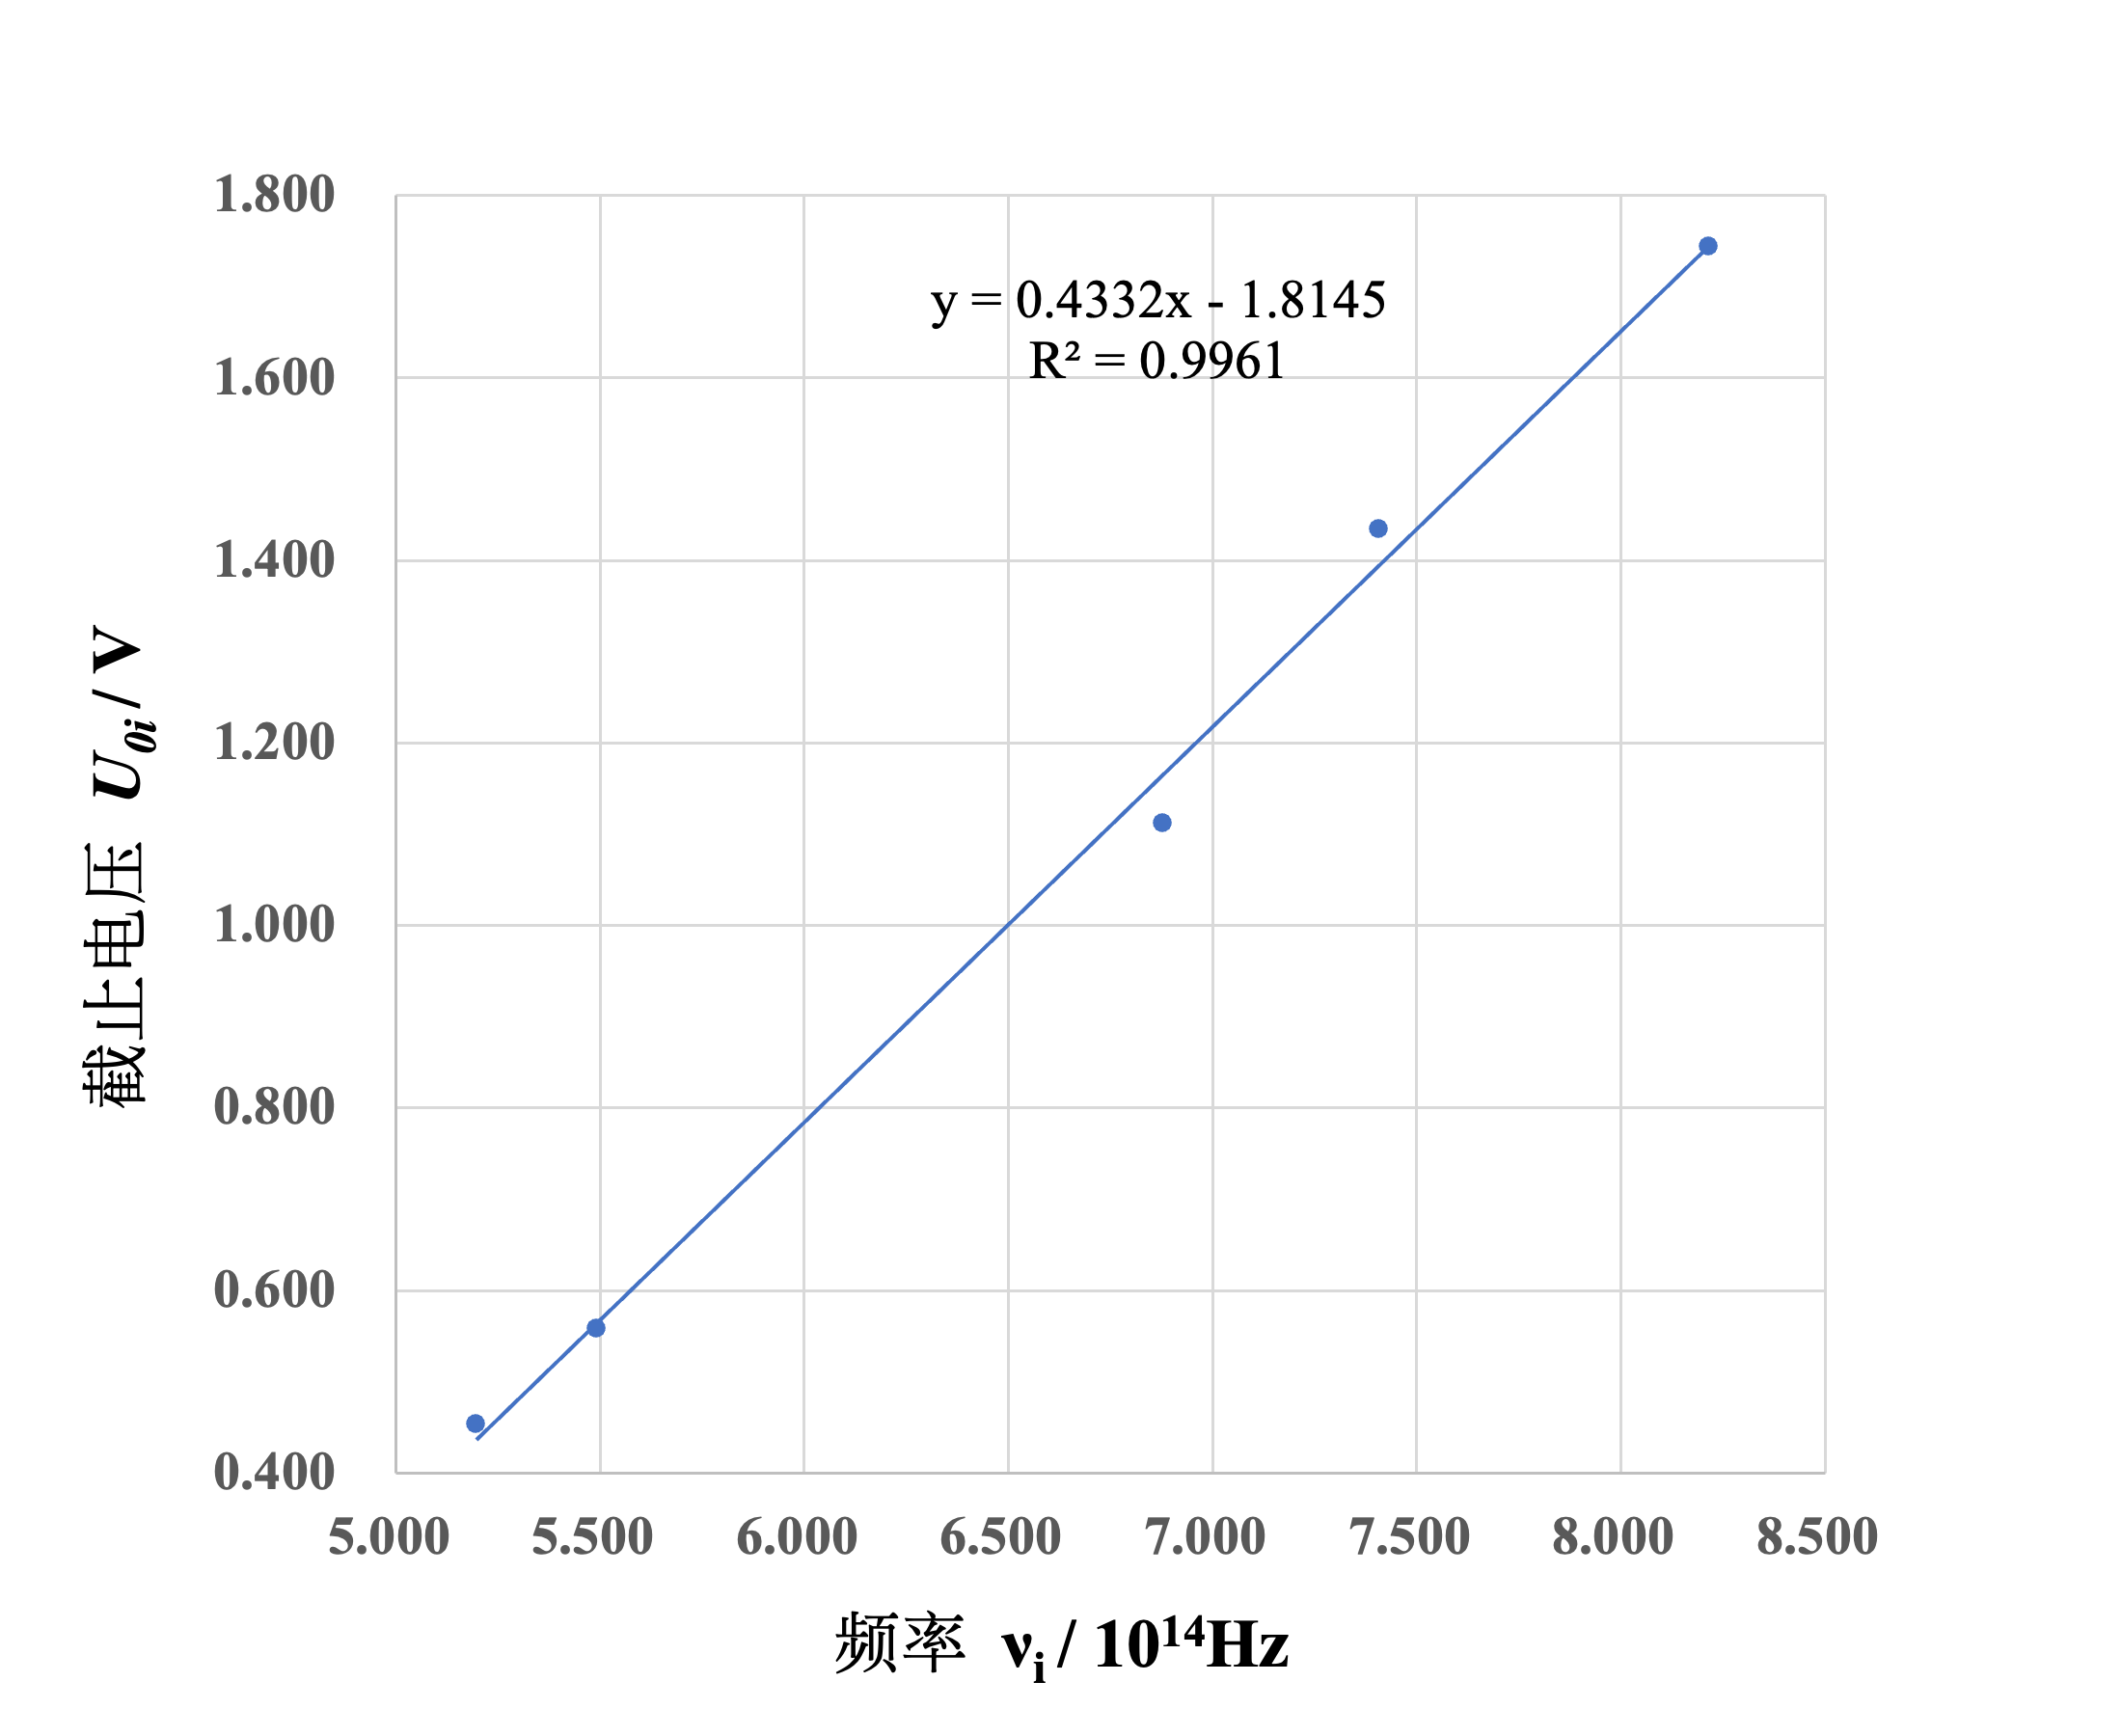
\includegraphics[width=0.9\linewidth]{tp1.png}
            \label{tp1.png}
        \end{minipage}
        \begin{minipage}{0.5\linewidth}
            \centering
            \textbf{图\ 6.2}\quad 补偿法测得截止电压与频率的$U-\nu$图 \\[4pt]
            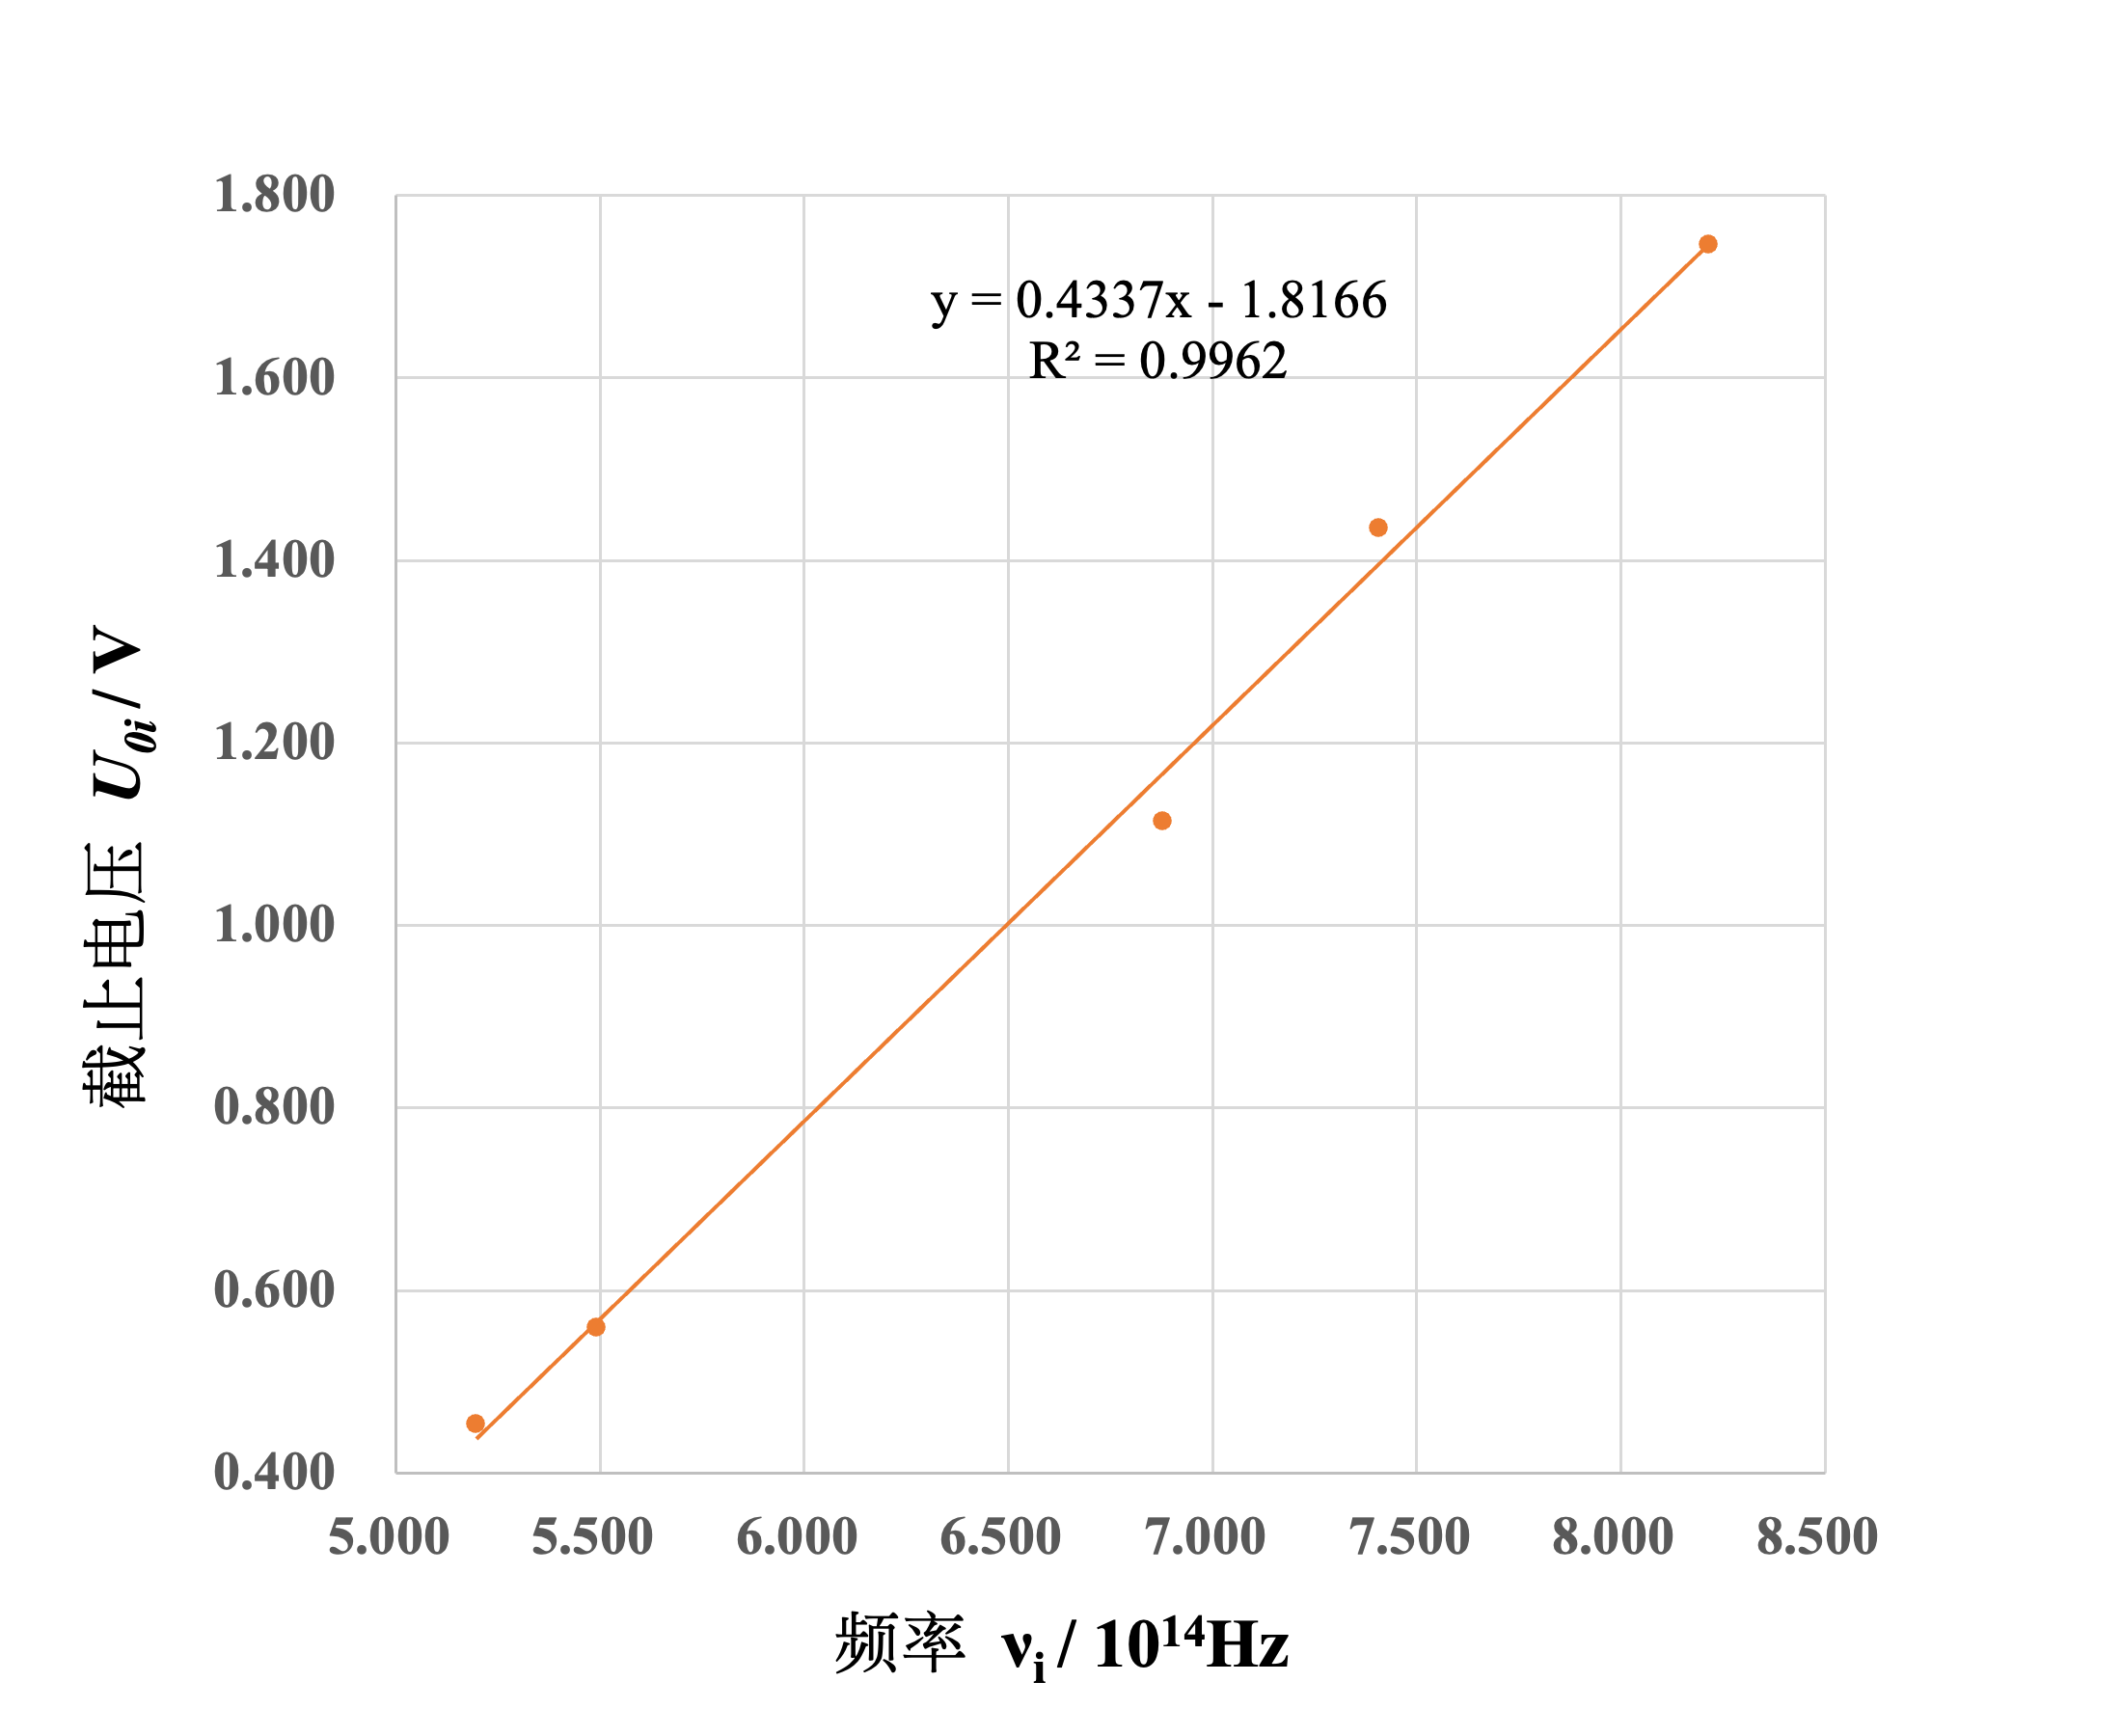
\includegraphics[width=0.9\linewidth]{tp2.png}
            \label{tp2.png}
        \end{minipage}\\[12pt]
        \kong (1)零点法：\\
        \kong $k=4.3332\times 10^{-15}J\cdot s\cdot C^{-1}$，$A=1.8145V$，$h=ek=6.9406\times 10^{-34}J\cdot s$，相对误差$\delta=4.74\%$\\
        \kong $\displaystyle \nu_{0}=\frac{A}{h}=2.614\times 10^{14}Hz$，$\displaystyle \lambda=\frac{c}{\nu}=1146.9nm$，$A_\text{逸出功}=A\cdot e=2.9068\times 10^{-19}V$\\[10pt]
        \kong (2)补偿法：\\
        \kong $k=4.3337\times 10^{-15}J\cdot s\cdot C^{-1}$，$A=1.8166V$$h=ek=6.9448\times 10^{-34}J\cdot s$，相对误差$\delta=4.81\%$\\
        \kong $\displaystyle \nu_{0}=\frac{A}{h}=2.616\times 10^{14}Hz$，$\displaystyle \lambda=\frac{c}{\nu}=1146.0nm$，$A_\text{逸出功}=A\cdot e=2.9102\times 10^{-19}V$\\
        \kong 可以看到，原理上补偿法应该更精确，但实际实验结果零点法略比补偿法相对误差较小，但两者对的误差都较大。\\

    \subsection{曲线法测量截止电压拟合计算普朗克常数}
        \kong 固定距离$L=400mm$，$\Phi=8mm$，通过测量多个点，绘制$I-U$曲线，数据如表6.2，绘制成图6.3：\\[12pt]
        \begin{minipage}{1\linewidth}
            \centering
            \textbf{表\ 6.2}\quad 光电管的伏安特性曲线测量  \\[4pt]
            \begin{tabular}{|l|l|l|l|l|l|l|l|l|l|l|l|}
                \hline
                \multirow{2}{*}{557.0nm} & $U_{AK}/V$    & -1.0   & -0.9   & -0.8   & -0.7   & -0.6   & -0.5  & -0.4  & -0.3  & -0.2 & -0.1  \\ \cline{2-12} 
                                         & $I/10^{-11}A$ & -33.2  & -32.5  & -31.8  & -31.0  & -28.1  & -20.1 & 9.5   & 88.4  & 218  & 376   \\ \hline
                \multirow{2}{*}{546.1nm} & $U_{AK}/V$    & -1.2   & -1.1   & -1.0   & -0.9   & -0.8   & -0.7  & -0.6  & -0.5  & -0.4 & -0.3  \\ \cline{2-12} 
                                         & $I/10^{-11}A$ & -43.0  & -42.0  & -40.9  & -39.9  & -37.6  & -33.5 & -22.4 & 10.0  & 93.0 & 229   \\ \hline
                \multirow{2}{*}{435.8nm} & $U_{AK}/V$    & -1.7   & -1.6   & -1.5   & -1.4   & -1.3   & -1.2  & -1.1  & -1.0  & -0.9 & -0.8  \\ \cline{2-12} 
                                         & $I/10^{-11}A$ & -149.7 & -141.9 & -133.5 & -120.4 & -102.7 & -75   & -11.7 & 113.2 & 308  & 648   \\ \hline
                \multirow{2}{*}{404.7nm} & $U_{AK}/V$    & -1.9   & -1.8   & -1.7   & -1.6   & -1.5   & -1.4  & -1.3  & -1.2  & -1.1 & -1.0  \\ \cline{2-12} 
                                         & $I/10^{-11}A$ & -73.7  & -66.3  & -58.6  & -45.3  & -25.7  & 4.0   & 51.5  & 125.2 & 239  & 423   \\ \hline
                \multirow{2}{*}{365.0nm} & $U_{AK}/V$    & -2     & -1.95  & -1.9   & -1.85  & -1.8   & -1.75 & -1.7  & -1.65 & -1.6 & -1.55 \\ \cline{2-12} 
                                         & $I/10^{-11}A$ & -57.5  & -50.9  & -43.4  & -35.7  & -25.3  & -11.5 & 9.5   & 41.0  & 87.1 & 147.6 \\ \hline
            \end{tabular}
        \end{minipage}\\[12pt]
        \begin{minipage}{1\linewidth}
            \centering
            \textbf{图\ 6.3}\quad 光电管的伏安特性曲线测量$I-U$图 \\[4pt]
            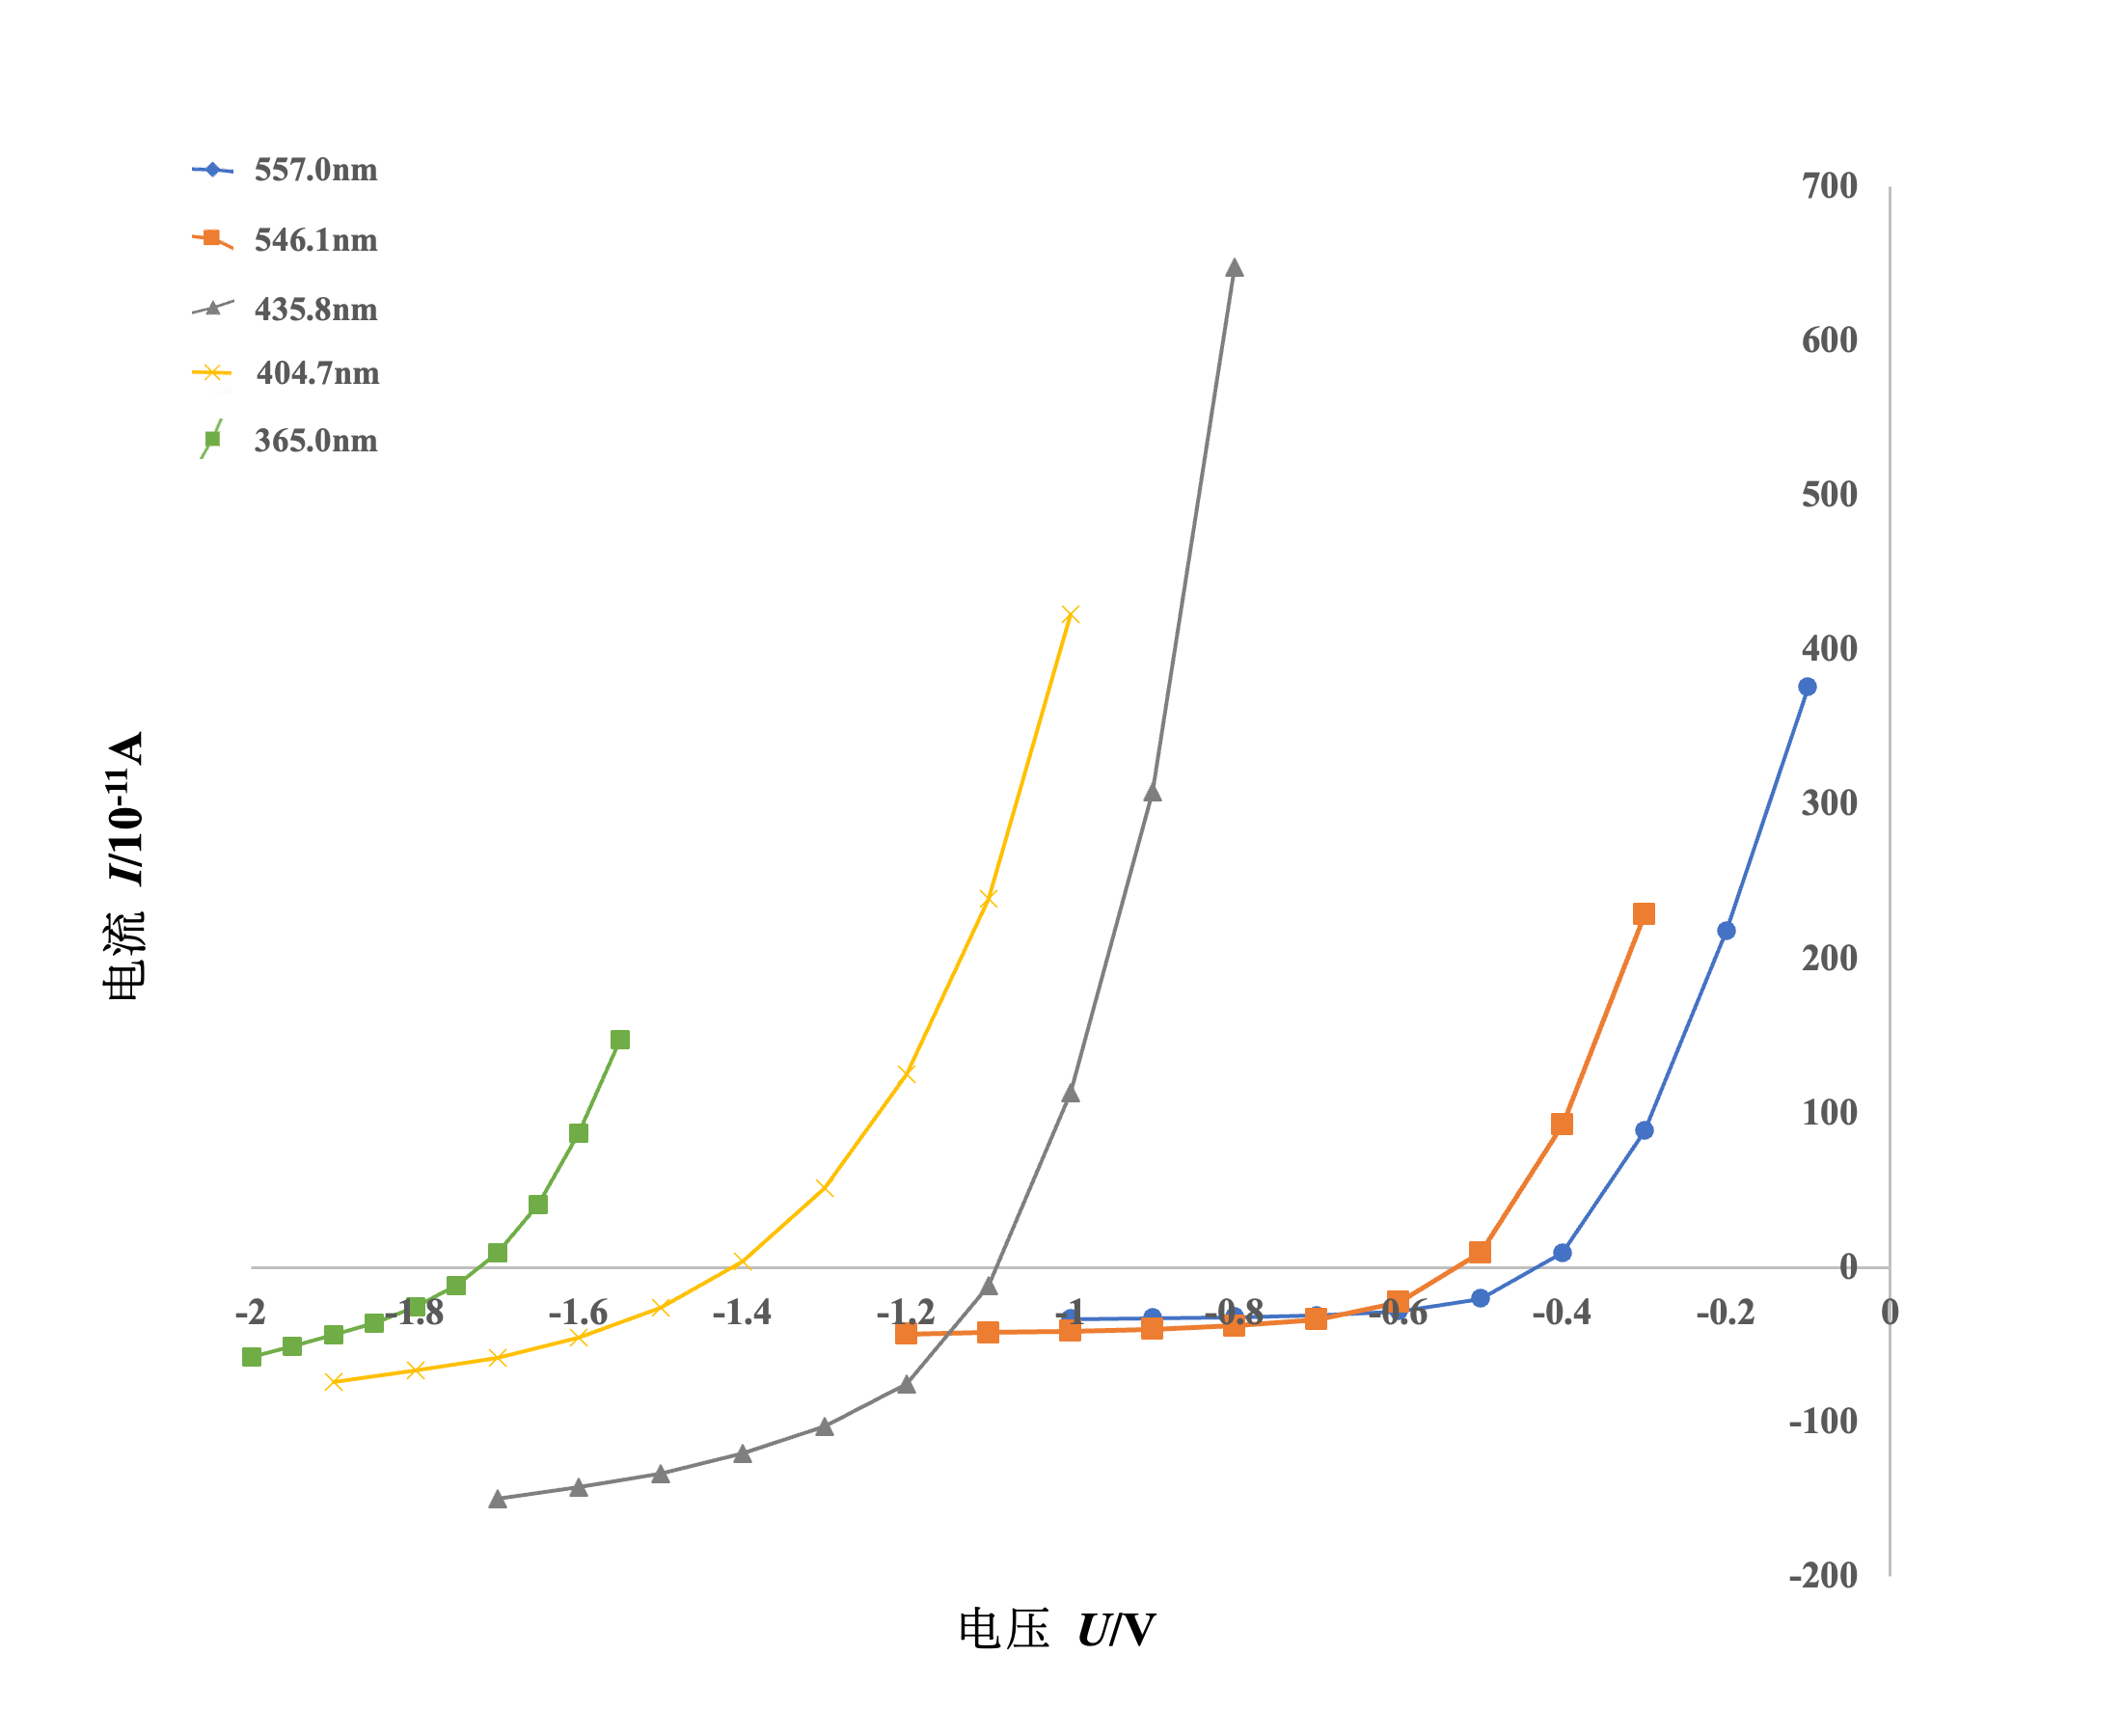
\includegraphics[width=0.9\linewidth]{tp3.png}
            \label{tp3.png}
        \end{minipage}\\[12pt]
        \kong 观察，得斜率突变时的电压即截止电压分别为$0.494V,\ 0.558V,\ 1.134V,\ 1.423V,\ 1.702V$。根据这些数据，再次描点连线，最小二乘法拟合，绘制$U-\nu$图，如图6.4：\\[12pt]
        \begin{minipage}{1\linewidth}
            \centering
            \textbf{图\ 6.4}\quad 测得截止电压与频率的$U-\nu$图 \\[4pt]
            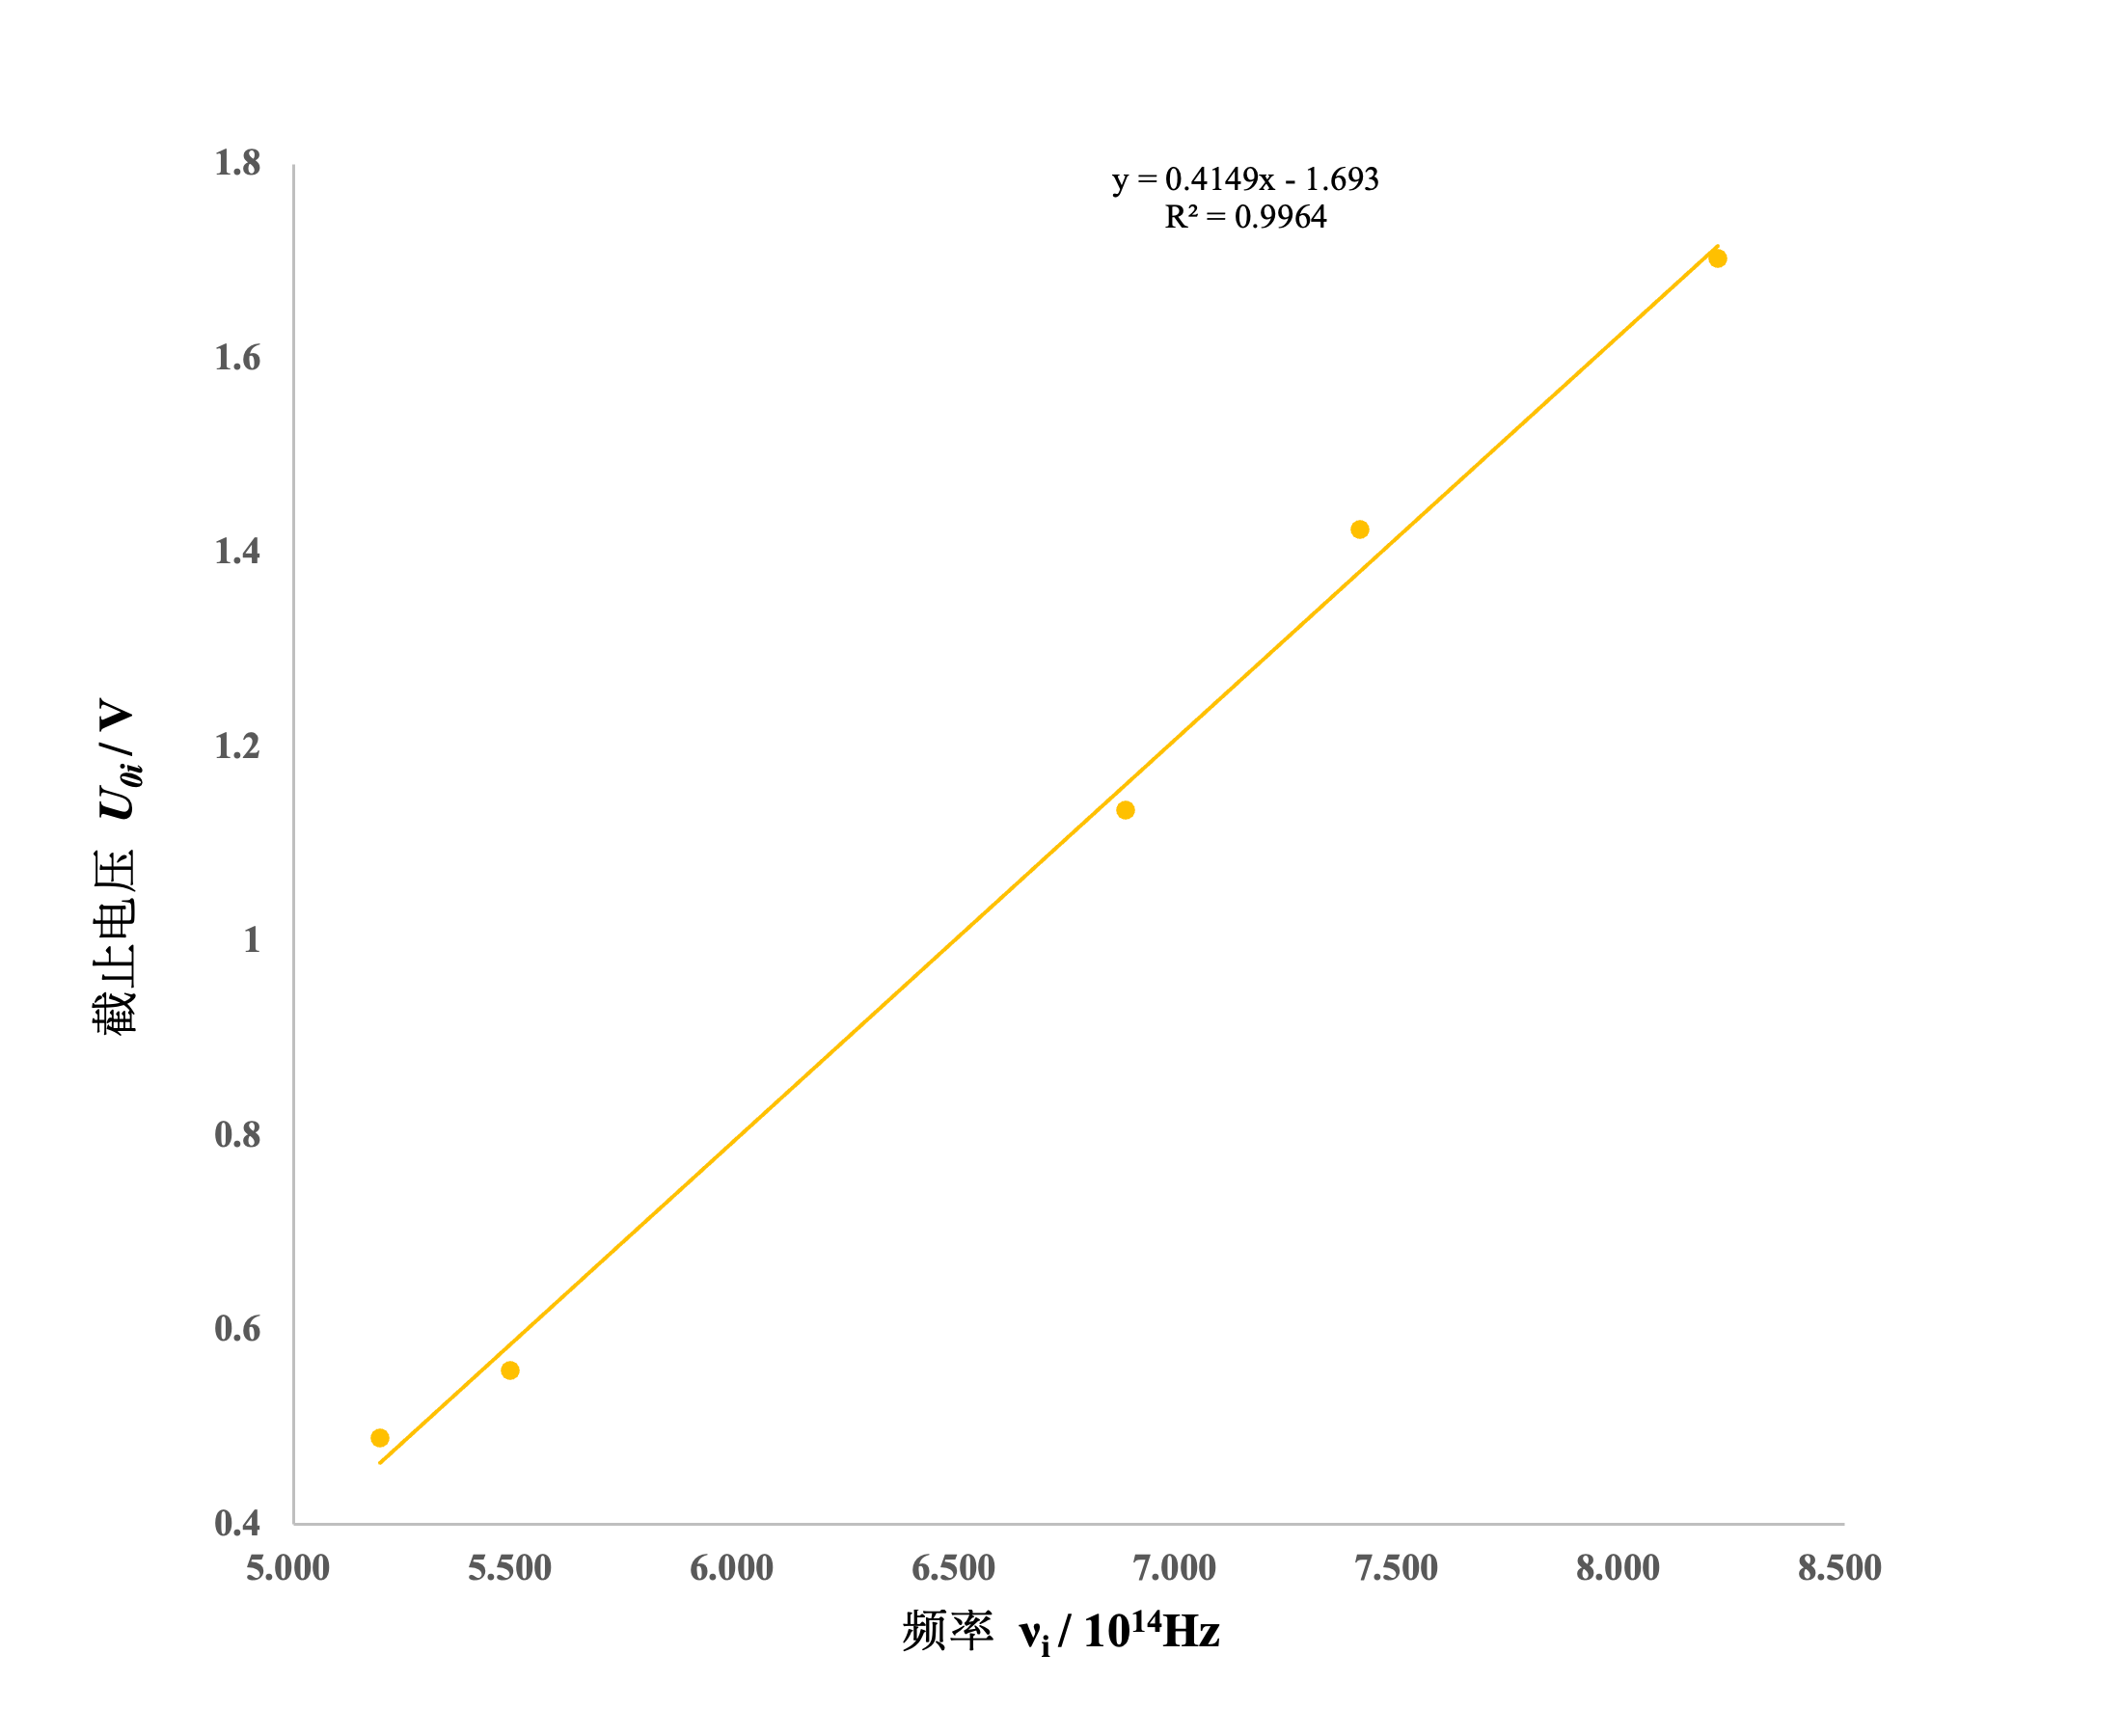
\includegraphics[width=0.9\linewidth]{tp4.png}
            \label{tp4.png}
        \end{minipage}\\[12pt]
        \kong $k=4.136\times 10^{-15}J\cdot s\cdot C^{-1}$，$A=1.583V$\\
        \kong $h=ek=6.6467\times 10^{-34}J\cdot s$，相对误差$\delta=0.31\%$\\
        \kong $\displaystyle \nu_{0,}=\frac{A}{h}=2.382\times 10^{14}Hz$，$\displaystyle \lambda=\frac{c}{\nu}=1258.6nm$\\
        \kong $A_\text{逸出功}=A\cdot e=2.53\times 10^{-19}V$\\
    
    \subsection{饱和光电流与光强的关系}
        \kong $U_{AK}=30V$下，分别固定距离($L=40.00cm$)改变光阑孔直径、固定光阑孔直径$\Phi=8mm$改变距离，从而改变光电流，数据如下表6.3，6.4：\\[12pt]
        \begin{minipage}{1\linewidth}
            \centering
            \textbf{表\ 6.3}\quad 固定距离改变光阑孔直径测得的光电流  \\[4pt]
            \begin{tabular}{|l|l|l|l|l|l|}
                \hline
                \multirow{2}{*}{435.8nm} & $\Phi/mm$     & 2    & 4    & 8     & 14.35 \\ \cline{2-6} 
                                         & $I/10^{-10}A$ & 7.86 & 29.9 & 118.6 & 401   \\ \hline
                \multirow{2}{*}{546.1nm} & $\Phi/mm$     & 2    & 4    & 8     & 14.35 \\ \cline{2-6} 
                                         & $I/10^{-10}A$ & 1.16 & 4.11 & 15.45 & 47.1  \\ \hline
            \end{tabular}
        \end{minipage}\\[12pt]
        \begin{minipage}{1\linewidth}
            \centering
            \textbf{表\ 6.4}\quad 固定光阑孔直径改变距离测得的光电流  \\[4pt]
            \begin{tabular}{|l|l|l|l|l|l|l|l|}
                \hline
                \multirow{2}{*}{435.8nm} & $L/cm$        & 30.00& 32.00& 34.00 & 36.00 & 38.00 & 40.00 \\ \cline{2-8} 
                                         & $I/10^{-10}A$ & 231  & 201  & 173.4 & 148.2 & 130.2 & 118.6 \\ \hline
                \multirow{2}{*}{546.1nm} & $L/cm$        & 30.00& 32.00& 34.00 & 36.00 & 38.00 & 40.00 \\ \cline{2-8} 
                                         & $I/10^{-10}A$ & 32.1 & 27.1 & 23.0  & 19.64 & 17.22 & 15.45 \\ \hline
            \end{tabular}
        \end{minipage}\\[12pt]
        使用最小二乘法拟合，制$I-\Phi^2$，$I-L^{-2}$散点图，如图6.5，6.6：\\[12pt]
        \begin{minipage}{0.5\linewidth}
            \centering
            \textbf{图\ 6.5}\quad $I-\Phi^2$图 \\[4pt]
            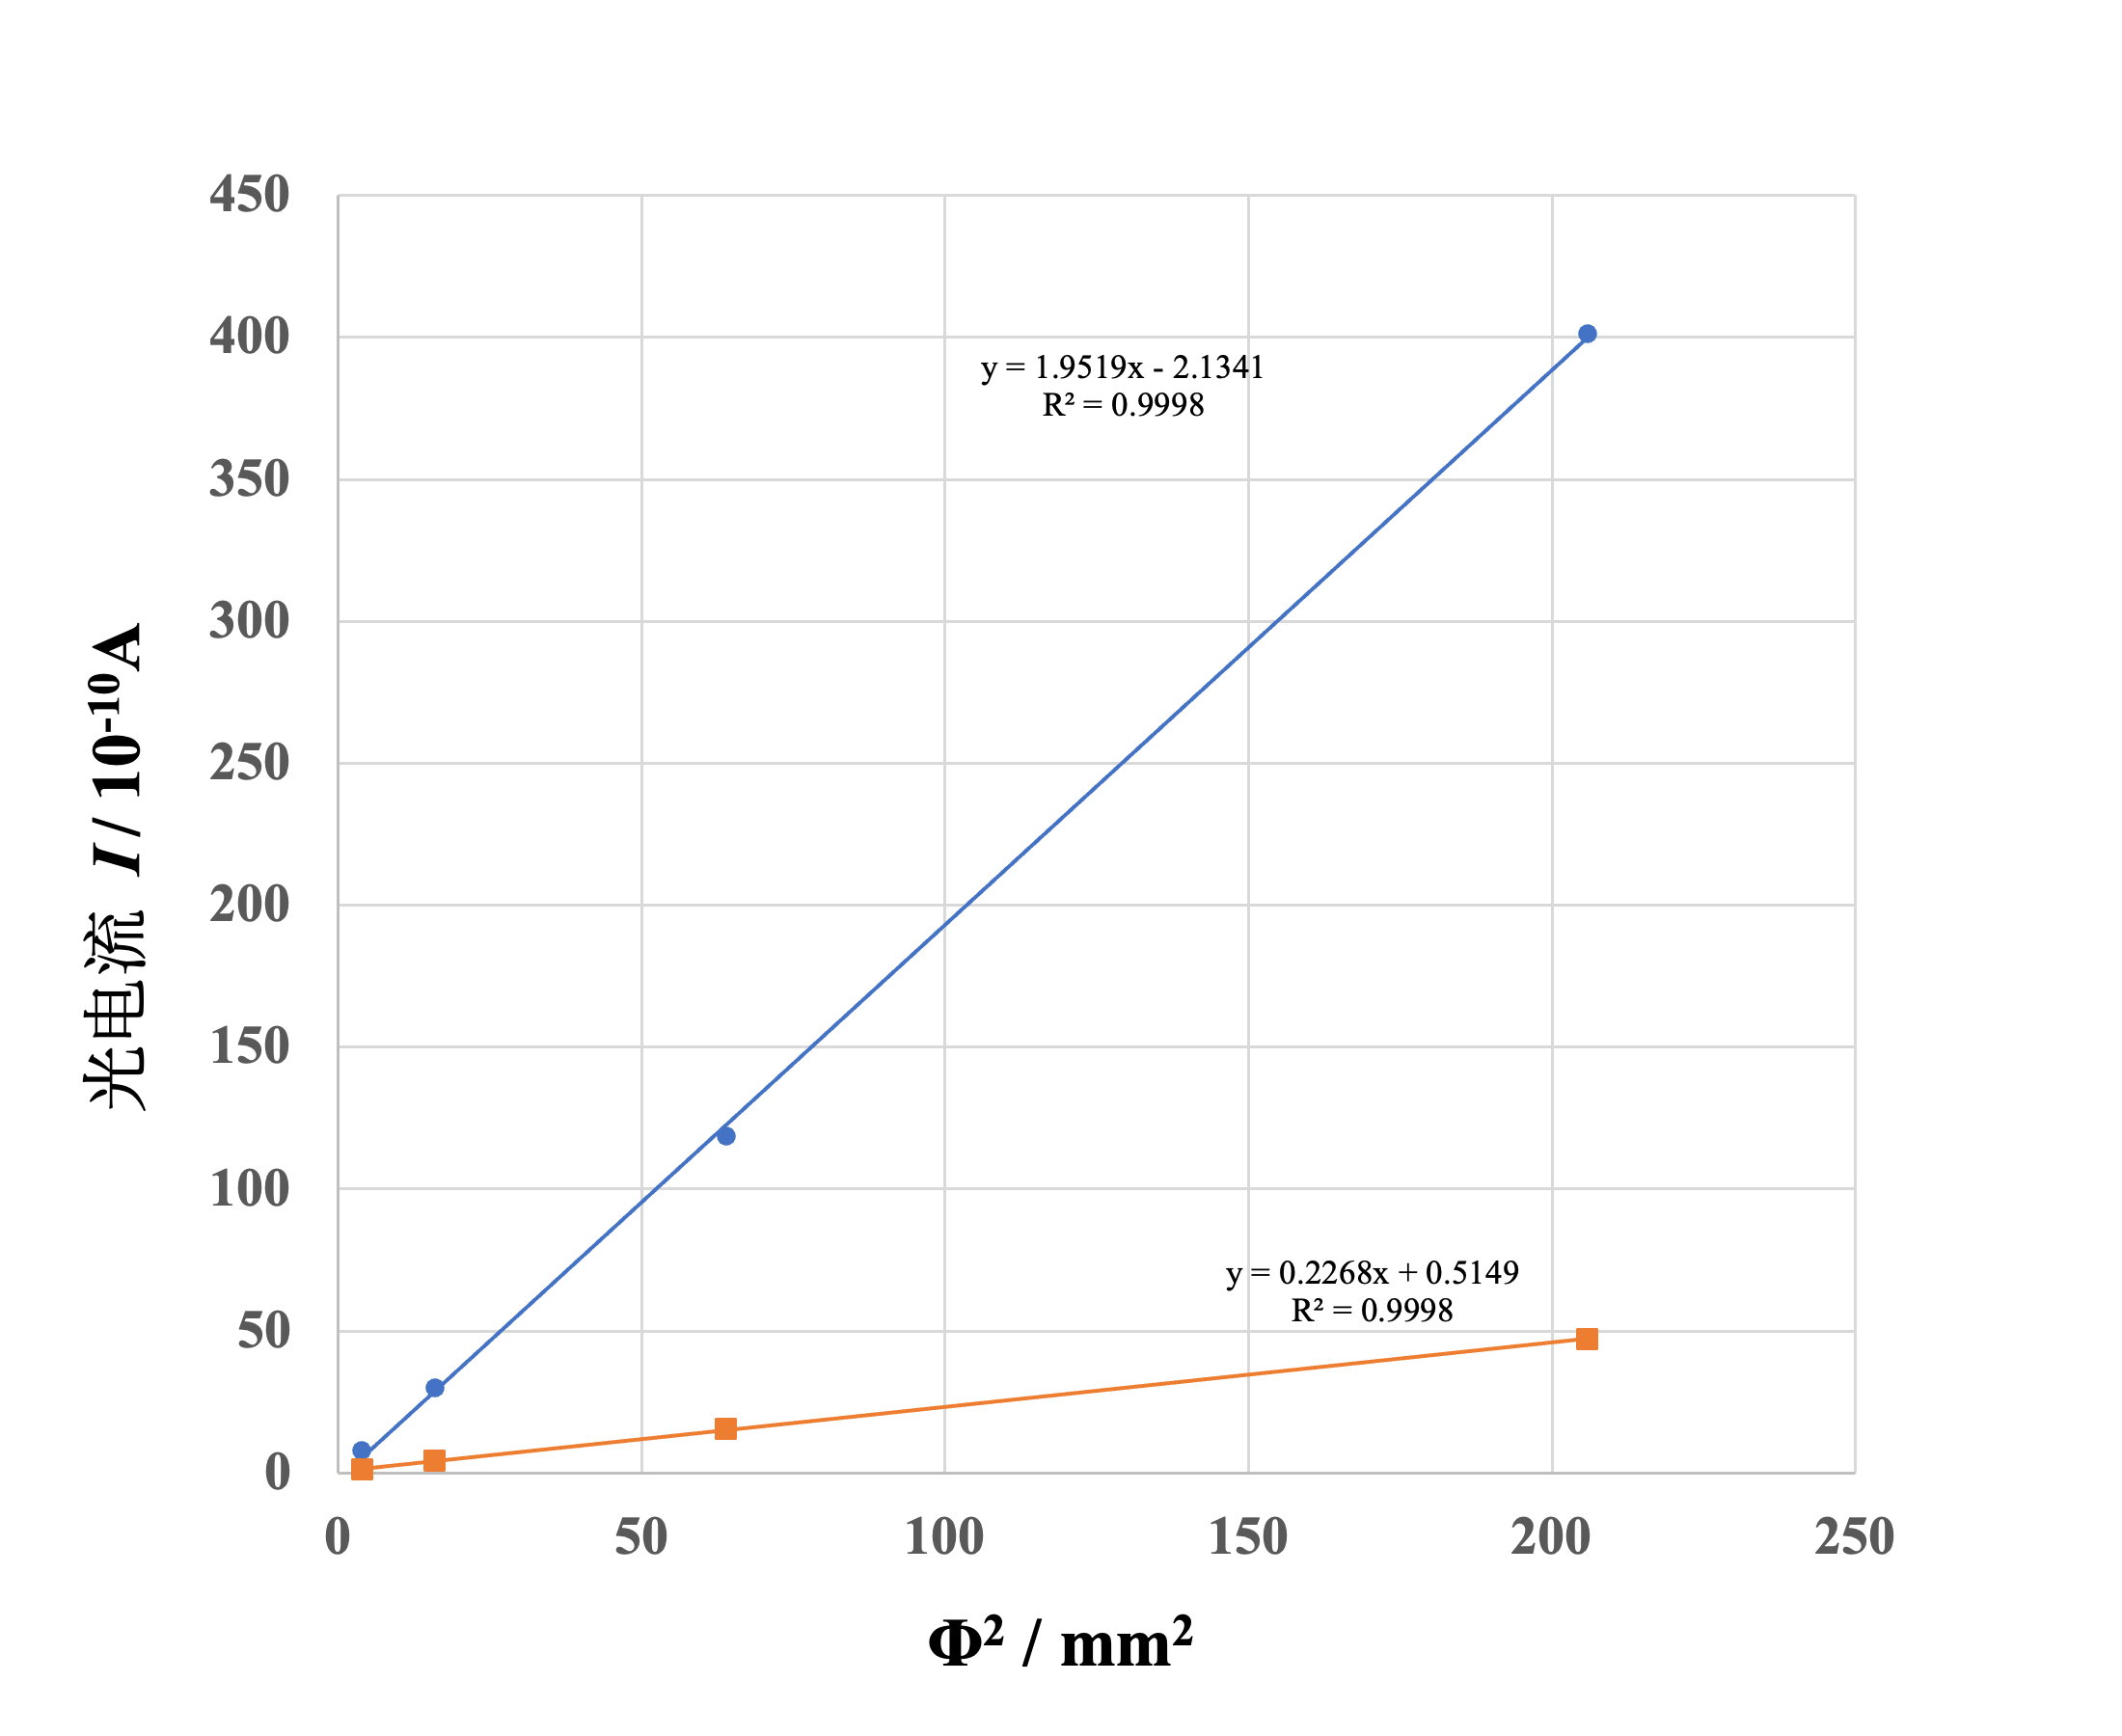
\includegraphics[width=0.9\linewidth]{tp5.png}
            \label{tp5.png}
        \end{minipage}
        \begin{minipage}{0.5\linewidth}
            \centering
            \textbf{图\ 6.6}\quad $I-L^{-2}$图 \\[4pt]
            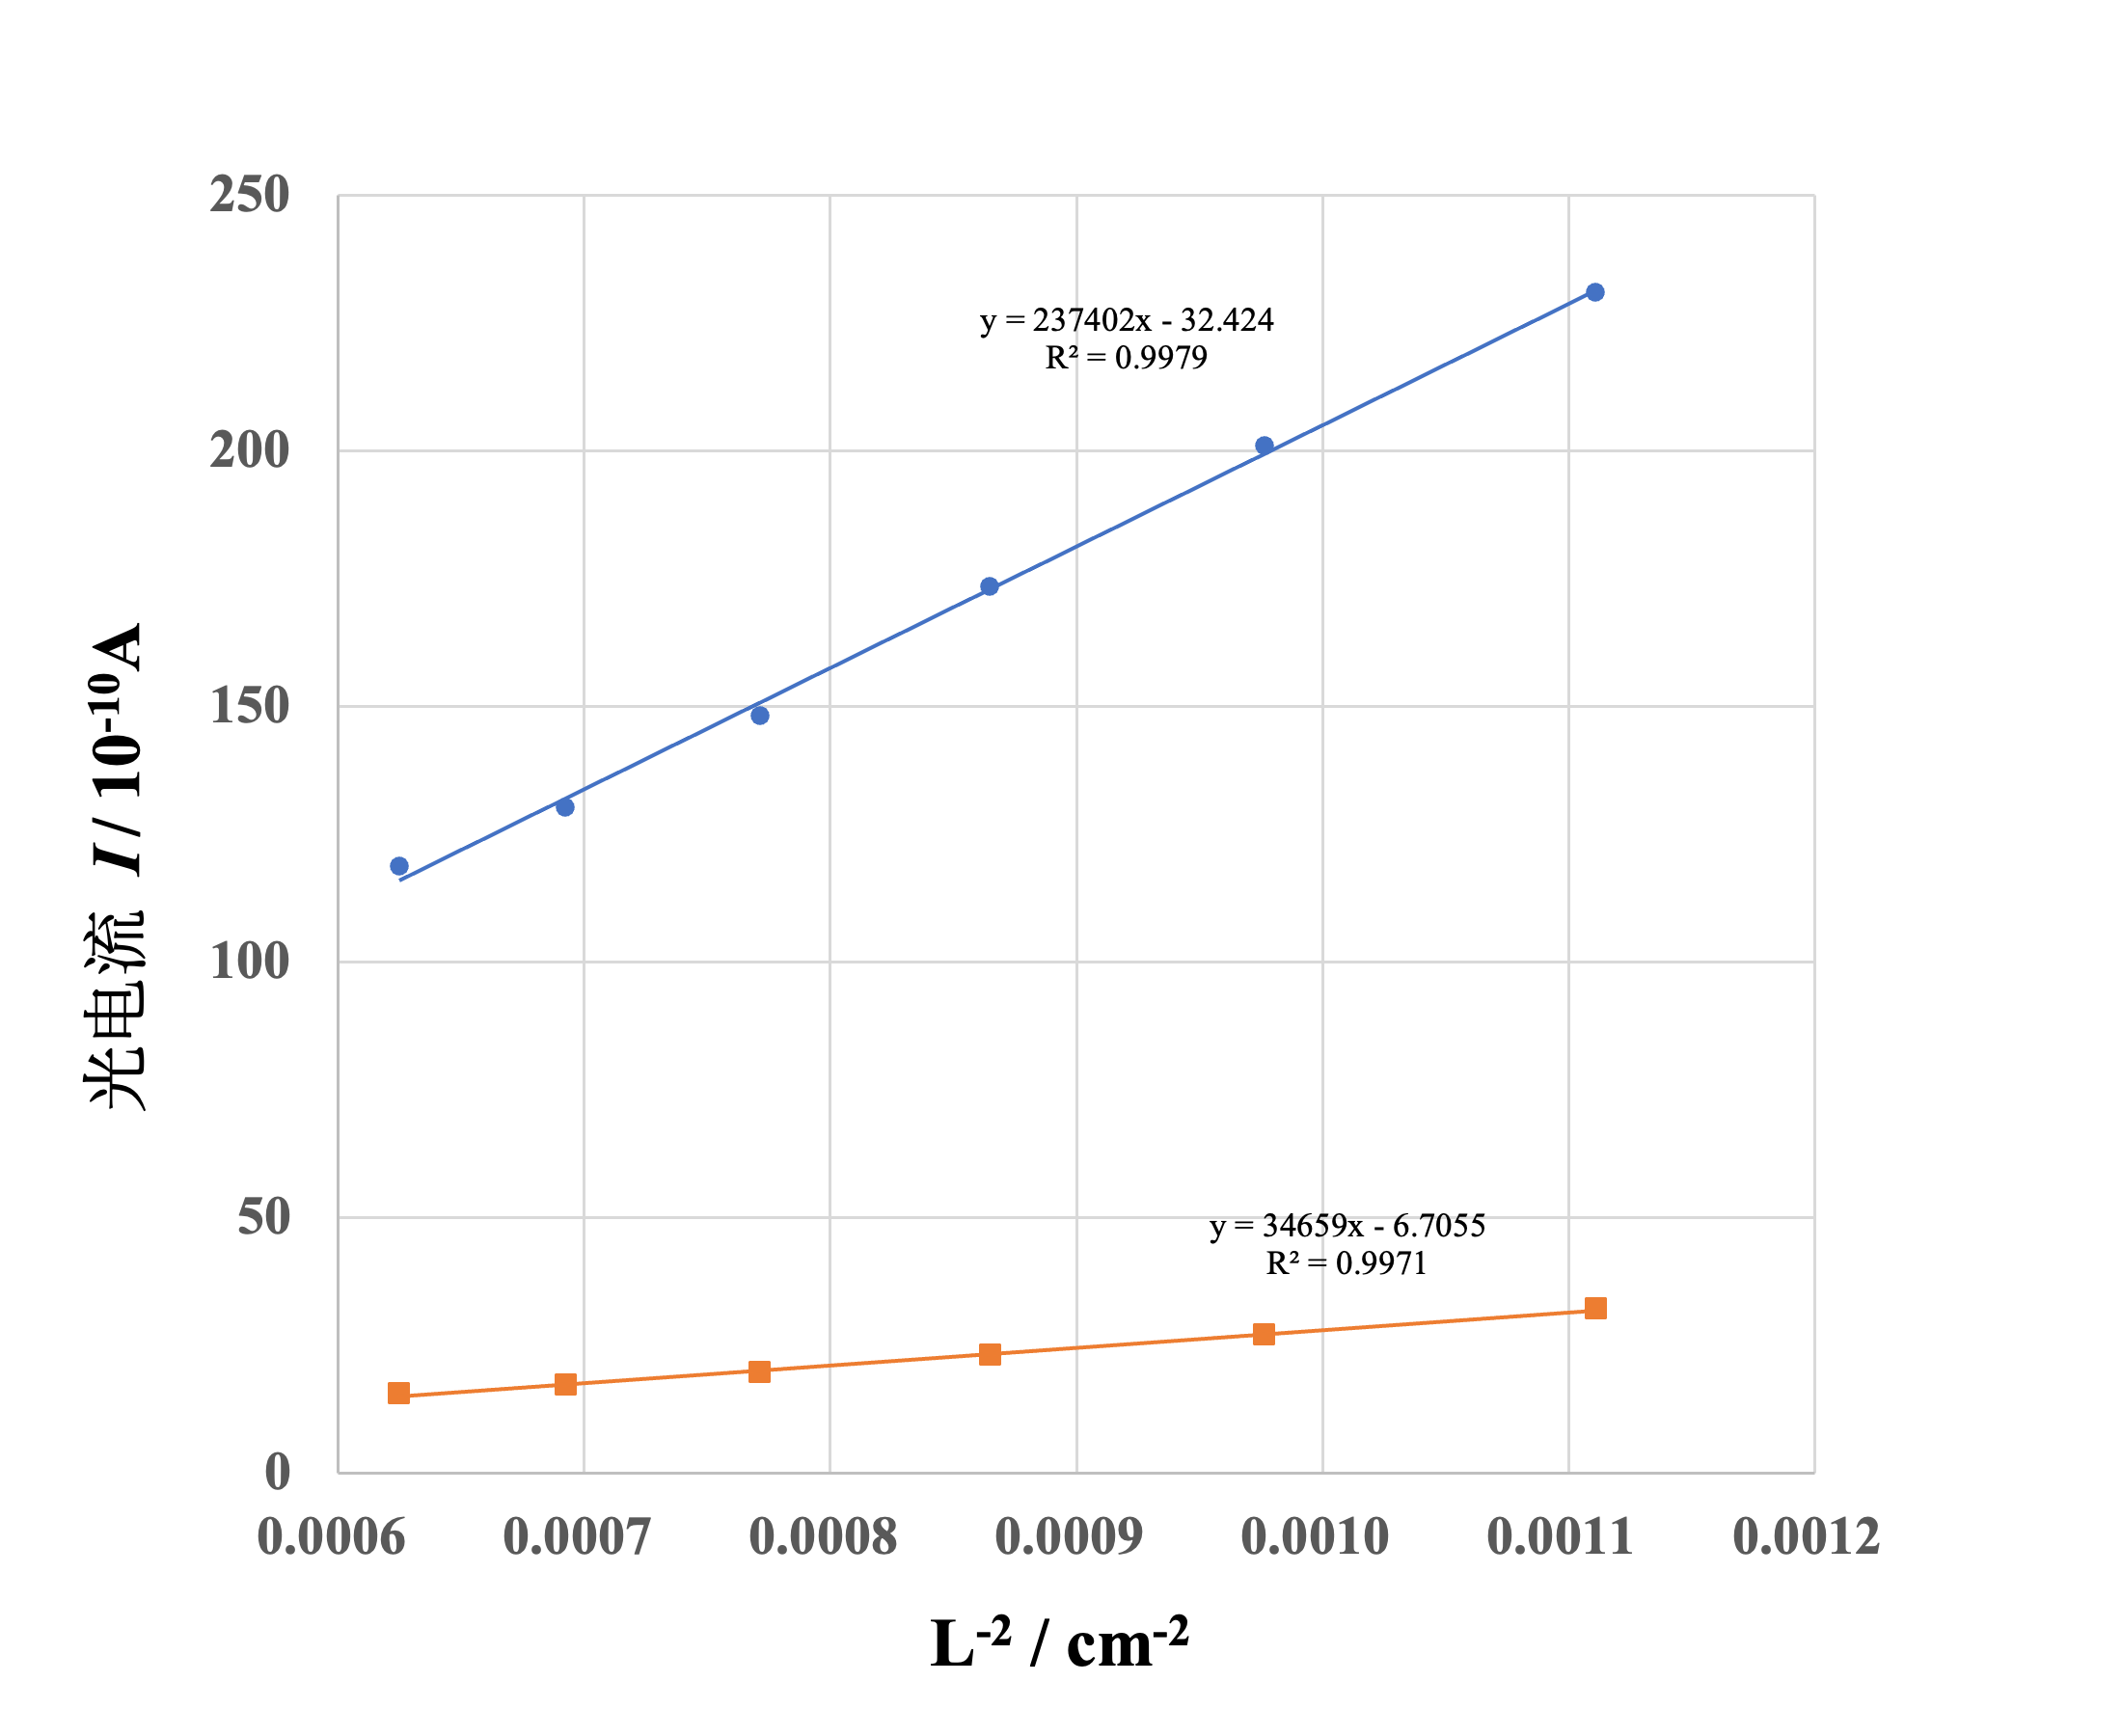
\includegraphics[width=0.9\linewidth]{tp6.png}
            \label{tp6.png}
        \end{minipage}\\[12pt]
        注意到$R^2$较接近$1$，基本呈线性关系，即光电流与光强在一定范围内呈线性关系。

\end{document}
